\subsection{Architecture}

In figure \ref{fig:architecture} a simple diagram of the architecture used from both Android application and Desktop application is shown. We used a \textit{Event Bus} architectural patter, in order to obtain a high decoupling degree between all the modules.

\begin{figure}[htbp]
	\centering
	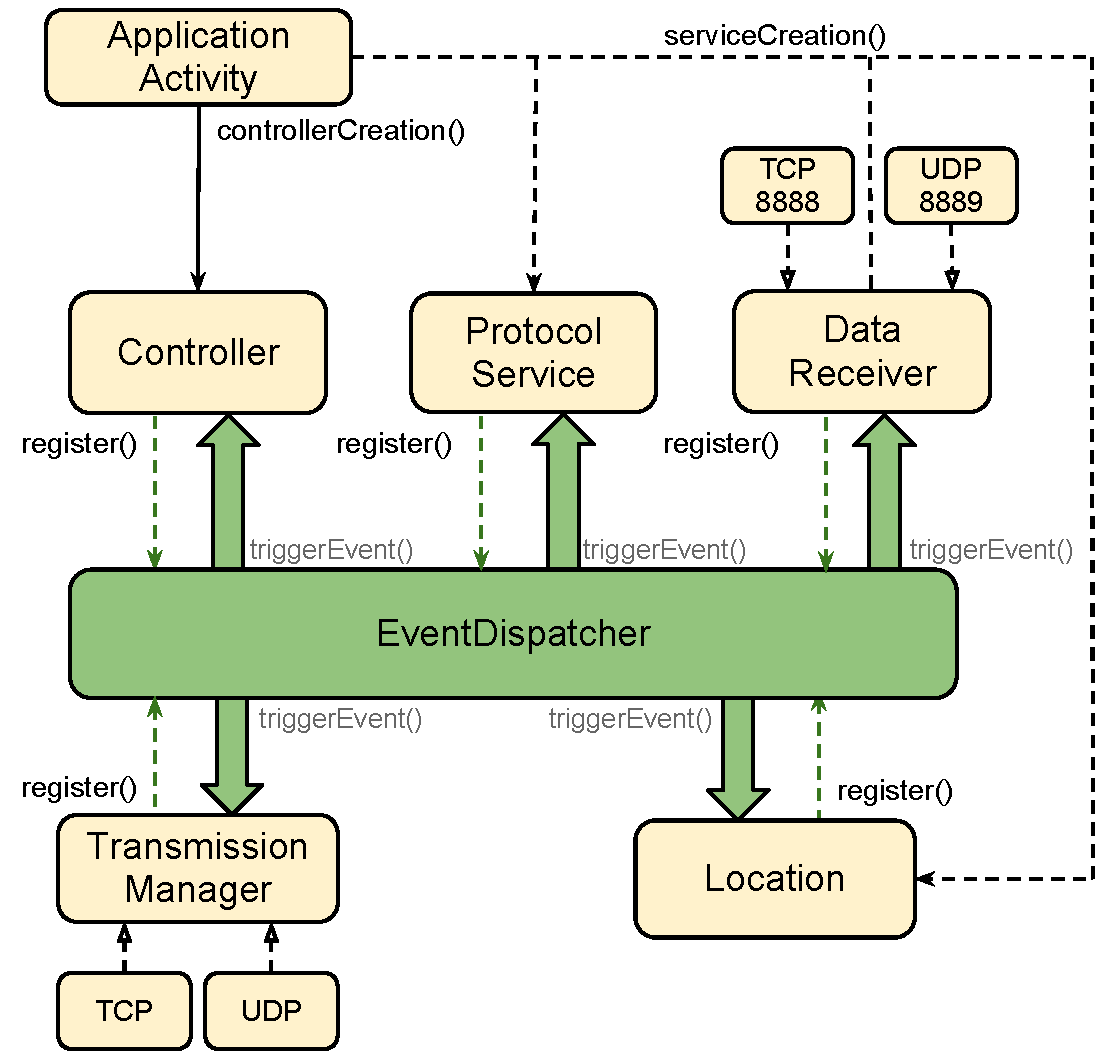
\includegraphics[trim = 10mm 0mm 0mm 0mm,width=3.5in]{imgs/components_architecture.pdf}
	\caption{Graphical representation of application structure.}
	\label{fig:architecture}
\end{figure}

This kind of architecture lets new algorithm modules to be tested, just registering them to the \textit{Event Bus} as \textit{Components}, listening for required events generated by GPS and WI-FI, and generating events to exchange data or to move to another position.

